\subsection{Montel spaces}

DEFINITION 4. --- A locally convex Hausdorff and barrelled space in which every bounded subset is relatively compact is called a Montel space.

Examples. --- 1) Every finite dimensional Hausdorff space is a Montel space. A normed space which is a Montel space is locally compact, hence is finite dimensional (I, p.~15, th. 3).

\begin{enumerate}
\def\labelenumi{\arabic{enumi})}
\setcounter{enumi}{1}
\tightlist
\item
  With the notations and hypothesis of prop. 7 of III, p.~6, the space E, being the inductive limit of Banach spaces, is barrelled (III, p.~25); moreover, every bounded subset of E is relatively compact (III, p.~6, prop. 7). In other words, E is a Montel space.
\end{enumerate}

In particular, Gevrey spaces (III, p.~10) are Montel spaces. * This is true for the space \(\mathcal{H}(\mathbf{K})\) consisting of germs of functions analytic in a neighbourhood of a compact subset \(\mathbf{K}\) of \(\mathbf{C}^n\) (III, p.~10).*

\begin{enumerate}
\def\labelenumi{\arabic{enumi})}
\setcounter{enumi}{2}
\tightlist
\item
  Every strict inductive limit E of a sequence \((\mathrm{E}_{n})\) of Montel spaces (II, p.~33) such that \(E_{n}\) is closed in \(E_{n+1}\) for all n, is a Montel space; in fact, E is Hausdorff (II, p.~32, prop. 9 (i)), barrelled (III, p.~25, cor. 3) and every bounded subset of E is contained in one of the \(E_{n}\) (III, p.~5, prop. 6) hence is relatively compact in \(E_{n}\) , and consequently also in E.
\end{enumerate}

* 4) Let U be an open set in \(\mathbf{R}^n\) and let \(\mathcal{C}^\infty (\mathrm{U})\) be the Fréchet space of infinitely differentiable functions on U (III, p.~9). We shall prove that this is a Montel space. Since \(\mathcal{C}^\infty (\mathrm{U})\) is a Fréchet space, it is barrelled (III, p.~25, corollary). Let B be a bounded subset of \(\mathcal{C}^\infty (\mathrm{U})\) and let K be a compact subset of U. For every \(\alpha \in \mathbf{N}^n\) let \(\mathrm{H}_{\alpha ,\mathrm{K}}\) be the set of restrictions to K of the functions \(\partial^{\alpha}f\) , as \(f\) runs through B. Let \(\alpha \in \mathbf{N}^n\) ; for every \(\beta \in \mathbf{N}^n\) such that \(|\beta | = |\alpha | + 1\) , the set \(\mathrm{H}_{\alpha ,\mathrm{K}}\) is bounded in \(\mathcal{C}(\mathbf{K})\) since B is bounded in \(\mathcal{C}^\infty (\mathrm{U})\) ; by VAR, R., No.~2.2.3, the set \(\mathrm{H}_{\alpha ,\mathrm{K}}\) is equicontinuous, hence (GT, X, § 2, No.~5)

relatively compact in \(\mathcal{C}(\mathbf{K})\) . But the topology of \(\mathcal{C}^{\infty}(\mathbf{U})\) is the coarsest among the topologies for which all the maps \(f\mapsto \partial^{\alpha}f|\mathbf{K}\) from \(\mathcal{C}^{\infty}(\mathbf{U})\) into \(\mathcal{C}(\mathbf{K})\) are continuous, therefore \(\mathbf{B}\) is relatively compact in \(\mathcal{C}^{\infty}(\mathbf{U})\) (GT, I, § 4, No.~1, prop. 3 and § 9, No.~5, corollary).

Similarly, the space \(\mathcal{C}_0^\infty (\mathrm{U})\) of all infinitely differentiable functions with compact support in U (III, p.~9) is a Montel space. For, \(\mathcal{C}_0^\infty (\mathrm{U})\) is the strict inductive limit of a sequence \(\mathcal{C}_{\mathrm{H}_n}^\infty (\mathrm{U})\) of Fréchet spaces (III, p.~9), and it is enough to see that each of the spaces \(\mathcal{C}_{\mathrm{H}_n}^\infty (\mathrm{U})\) is a Montel space (Example 3). But a bounded and closed subset of \(\mathcal{C}_{\mathrm{H}_n}^\infty (\mathrm{U})\) is closed and bounded in \(\mathcal{C}^{\infty}(\mathrm{U})\) , hence compact in \(\mathcal{C}^{\infty}(\mathrm{U})\) , and consequently in \(\mathcal{C}_{\mathrm{H}_n}^\infty (\mathrm{U})\) .

PROPOSITION 8. --- Let E be a Montel space and F a filter on E, which converges to a point \(x_{0}\) in E for the weakened topology. If F is a countable base, or contains a bounded set, then F, converges to \(x_{0}\) for the initial topology also.

Assume first that there exists a bounded set B in F. The closure \(\overline{B}\) of B for the initial topology of E is bounded; in addition, \(\overline{B}\) is compact because E is a Montel space. The topology on \(\overline{B}\) induced by \(\sigma(E, E')\) is Hausdorff and coarser than the topology induced by the initial topology; they therefore coincide (GT, I, § 9, No.~4). This proves the proposition for this case.

Next assume that \(\mathfrak{F}\) has a countable base. It is enough (GT, I, §6, No.~8, prop. 11) to consider the case of a sequence \((x_{n})_{n\geqslant 1}\) tending to \(x_0\) for \(\sigma (\mathrm{E},\mathrm{E}^{\prime})\) . Let B be the set of all \(x_{n}\) for \(n\geqslant 0\) . This set is bounded for \(\sigma (\mathrm{E},\mathrm{E}^{\prime})\) , hence also for the initial topology (III, p.~27, cor. 3). Thus we have reduced to the first case of the proof.

Every Montel space is reflexive : this follows from def. 4 and from th. 2 of IV, p.~16. Further :

PROPOSITION 9. --- The strong dual of a Montel space is a Montel space.

Let E be a Montel space and \(E_{b}^{\prime}\) its strong dual. Since E is reflexive, \(E_{b}^{\prime}\) is barrelled (IV, p.~15, th. 1). Since every bounded subset of E is relatively compact the strong topology on \(E^{\prime}\) coincides with the topology of compact convergence. Let B be a bounded subset of \(E_{b}^{\prime}\) ; it is bounded for the weak topology \(\sigma(E^{\prime}, E)\) , hence is equicontinuous because E is barrelled. Then Ascoli's theorem (GT, X, § 2, No.~4, cor. and § 2, No.~5, cor. 1) implies that the closure of B for \(\sigma(E^{\prime}, E)\) is compact for the topology of compact convergence; therefore B is relatively compact in \(E_{b}^{\prime}\) .

PROPOSITION 10. --- Every metrizable Montel space satisfies the first axiom of countability.

Let E be a metrizable Montel space. We know (II, p.~5) that E can be identified with a subspace of the product \(F = \prod_{n \in N} F_n\) of a sequence of normed spaces, and we can even assume that we have \(\Pr_n(E) = F_n\) for all \(n \in N\) . If each of the metrizable spaces \(F_n\) satisfies the first axiom of countability, then so does F (GT, IX, § 2, No.~8), hence also E.

We argue by reductio ad absurdum. Assume for example that \(F_{0}\) does not satisfy the first axiom of countability. Let \(B_{0}\) be the unit ball (closed) in \(F_{0}\) ; this is a metric space which does not satisfy the first axiom of countability. We shall use the following lemma :

Lemma 1. --- Suppose the metric space X does not satisfy the first axiom of countability. Then there exists a real number \(\varepsilon > 0\) and an uncountable subset A in X such that \(d(x, y) \geqslant \varepsilon\) for all distinct \(x, y\) in A.

For every integer \(n \geqslant 1\) , let \(\mathfrak{F}_n\) be the set (ordered by inclusion) of subsets \(D\) of \(X\) such that \(d(x, y) \geqslant \frac{1}{n}\) for distinct \(x, y\) in \(D\) . The set \(\mathfrak{F}_n\) is of finite character, hence possesses a maximal element \(D_n(S, III, \S 4, No. 5)\) . Then for all \(y \in X\) , there exists a point \(x\) in \(D_n\) such that \(d(x, y) < \frac{1}{n}\) , by virtue of the maximal character of \(D_n\) . Put \(D = \bigcup_{n} D_n\) ; the set \(D\) is then dense in \(X\) , and since \(X\) does not satisfy the first axiom of countability, \(D\) is not countable, and so one of the \(D_n\) is not countable.

Q.E.D.

By lemma 1, applied to \(\mathbf{B}_0\) , there exists an uncountable subset \(\mathbf{A}_0\) of \(\mathbf{F}_0\) and a number \(\varepsilon > 0\) such that \(\| x \| \leqslant 1\) and \(\| x - y \| \geqslant \varepsilon\) for distinct \(x, y\) in \(\mathbf{A}_0\) . We have \(\mathrm{pr}_0(\mathrm{E}) = \mathrm{F}_0\) and hence there exists a subset \(\mathbf{A}\) in \(\mathbf{E}\) such that \(\mathrm{pr}_0\) induces a bijection from \(\mathbf{A}\) onto \(\mathbf{A}_0\) .

Lemma 2. --- There exists a sequence \((x_{m})_{m\geqslant 0}\) consisting of distinct elements of A, which is bounded in E.

We shall construct a sequence \((x_{m})_{m\geqslant 0}\) of points of A by induction; and a decreasing sequence \((\mathrm{C}_m)_{m\geqslant 0}\) of subsets of A satisfying the following conditions:

\begin{enumerate}
\def\labelenumi{\alph{enumi})}
\item
  None of the sets \(\mathbf{C}_m\) is countable.
\item
  For every \(n \geqslant 0\) , the set \(\mathrm{pr}_k(\mathbf{C}_m)\) is bounded in \(\mathbf{F}_k\) for \(0 \leqslant k \leqslant m\) .
\item
  For every \(m \geqslant 0\) , we have \(x_{m} \in \mathbf{C}_{m} - \mathbf{C}_{m+1}\) .
\end{enumerate}

We put \(C_0 = A\) . Suppose the sets \(C_m\) for \(0 \leqslant m \leqslant n\) have been defined, so as to satisfy a) and b) for \(0 \leqslant m \leqslant n\) , and also the points \(x_m\) in \(C_m - C_{m+1}\) for \(0 \leqslant m < n\) . For every integer \(r \geqslant 1\) , let \(C_{n,r}\) be the set of all \(x \in C_n\) such that

\[
r - 1 \leqslant \left\| \operatorname{pr} _ {n + 1} (x) \right\| <   r.
\]

Since \(\mathbf{C}_n\) is not countable, there exists an integer \(r \geqslant 1\) such that \(\mathbf{C}_{n,r}\) is not countable. We choose a point \(x_n\) in \(\mathbf{C}_{n,r}\) and put \(\mathbf{C}_{n+1} = \mathbf{C}_{n,r} - \{x_n\}\) . Evidently \(\mathbf{C}_{n+1} \subset \mathbf{C}_n\) and \(x_n \in \mathbf{C}_n - \mathbf{C}_{n+1}\) , the set \(\mathbf{C}_{n+1}\) is not countable and \(\mathrm{pr}_k(\mathbf{C}_{n+1})\) is bounded in \(\mathbf{F}_n\) for \(0 \leqslant k \leqslant n + 1\) .

We have \(x_{m} \in C_{m}\) , and so \(x_{m} \in C_{n}\) where \(m \geqslant n\) . The projection of the sequence \((x_{m})_{m \geqslant 0}\) on \(F_{n}\) is therefore bounded for all \(n \geqslant 0\) ; in other words, the sequence \((x_{m})_{m \geqslant 0}\) is bounded in E, and this establishes lemma 2.

Q.E.D.

With the notations of lemma 2, the bounded sequence \((x_{m})_{m\geqslant 0}\) has a limit point \(y\) in E. Therefore the sequence \((\mathrm{pr}_0(x_m))_{m\geqslant 0}\) has a limit point \(\mathrm{pr}_0(y)\) in \(\mathbf{F}_0\) , but this contradicts the construction of \(\mathbf{A}_0\) .

COROLLARY. --- Let E be a metrizable Montel space. Then there exists a countable dense set in the strong dual of E.

On the dual \(E'\) of E, the strong topology is identical with that of compact convergence, since E is a Montel space. It is now enough to apply cor. 1 of prop. 6 of III, p.~18.

\pandocbounded{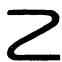
\includegraphics[keepaspectratio]{images/part002_3e739bde.jpg}}

We can show that the strong dual of a metrizable Montel space \(E\) is not metrizable if \(E\) is infinite dimensional (IV, p.~57, exerc. 1).

